\everymath{\displaystyle}
\documentclass{beamer}
% \documentclass[handout]{beamer}

%\usepackage[pdftex]{color,graphicx}
\usepackage{amsmath,amssymb,amsfonts}

\mode<presentation>
{
  % \usetheme{Darmstadt}
  % \usetheme[hideothersubsections]{Hannover}
  % \usetheme[hideothersubsections]{Goettingen}
  \usetheme[hideothersubsections, right]{Berkeley}

  \usecolortheme{seahorse}
  % \usecolortheme{dolphin}
  \usecolortheme{rose}
  % \usecolortheme{orchid}

  \useinnertheme[shadow]{rounded}

  \setbeamercovered{transparent}
  % or whatever (possibly just delete it)
}

\mode<handout>{
  \setbeamercolor{background canvas}{bg=black!5}
  \usepackage{pgfpages}
  \pgfpagesuselayout{4 on 1}[a4paper,border shrink=5mm, landscape]
}

\usepackage[brazilian]{babel}
% or whatever

% \usepackage[latin1]{inputenc}
\usepackage[utf8]{inputenc}
% or whatever

\usepackage{times}
%\usepackage[T1]{fontenc}
% Or whatever. Note that the encoding and the font should match. If T1
% does not look nice, try deleting the line with the fontenc.


\title%[] % (optional, use only with long paper titles)
{Tópicos de Escrita Científica}

\subtitle
{} % (optional)

\author%[] % (optional, use only with lots of authors)
{Felipe Figueiredo}% \and S.~Another\inst{2}}
% - Use the \inst{?} command only if the authors have different
%   affiliation.

\institute[INTO] % (optional, but mostly needed)
{Instituto Nacional de Traumatologia e Ortopedia
}
  % \inst{1}%
  % Department of Computer Science\\
  % University of Somewhere
  % \and
  % \inst{2}%
  % Department of Theoretical Philosophy\\
  % University of Elsewhere}
% - Use the \inst command only if there are several affiliations.
% - Keep it simple, no one is interested in your street address.

\date%[] % (optional)
{}

% \subject{Talks}
% This is only inserted into the PDF information catalog. Can be left
% out. 



% If you have a file called "university-logo-filename.xxx", where xxx
% is a graphic format that can be processed by latex or pdflatex,
% resp., then you can add a logo as follows:

\pgfdeclareimage[height=1.6cm]{university-logo}{../logo}
\logo{\pgfuseimage{university-logo}}



% Delete this, if you do not want the table of contents to pop up at
% the beginning of each subsection:
\AtBeginSubsection[]
%\AtBeginSection[]
{
  \begin{frame}<beamer>{Sumário}
    \tableofcontents[currentsection,currentsubsection]
  \end{frame}
}


% If you wish to uncover everything in a step-wise fashion, uncomment
% the following command: 

% \beamerdefaultoverlayspecification{<+->}


\begin{document}

\begin{frame}
  \titlepage
\end{frame}

\begin{frame}{Sumário}
  \tableofcontents
  % You might wish to add the option [pausesections]
\end{frame}


%% Template
% \section{}

% \subsection{}

% \begin{frame}{}
%   \begin{itemize}
%   \item 
%   \end{itemize}
% \end{frame}

% \begin{frame}
%   \begin{columns}
%     \begin{column}{5cm}
%     \end{column}
%     \begin{column}{5cm}
%     \end{column}
%   \end{columns}
% \end{frame}

% \begin{frame}{}
%   \includegraphics[height=0.4\textheight]{file1}
%   \includegraphics[height=0.4\textheight]{file2}
%   \includegraphics[height=0.4\textheight]{file3}
%   \begin{figure}
%     \caption{}
%   \end{figure}
% \end{frame}

% \begin{frame}{}
%   \begin{definition}
%   \end{definition}
%   \begin{example}
%   \end{example}
%   \begin{block}{Exercício}
%   \end{block}
% \end{frame}

\section{Discussão da aula passada}

% \subsection{Discussão da aula passada}

\begin{frame}{Discussão da aula passada}
  \begin{block}{}
    Discussão da leitura obrigatória da aula passada
  \end{block}
\end{frame}

\section{Estrutura do texto}

\subsection{Expectativas do leitor}

\begin{frame}{As necessidades do leitor}
  \begin{block}{Gopen e Swan, 1990}
    ``Para o leitor apreender o que o autor quer dizer, o autor
    precisa entender o que o leitor precisa.''
  \end{block}\pause
  \begin{block}{Hindle, 2013}
    ``Você não está escrevendo para você mesmo, está escrevendo para
    seu leitor.''
  \end{block}\pause
  \begin{block}{Figueiredo, hoje.}
    ``O \alert{trabalho} da comunicação é seu, não do leitor.''
  \end{block}
\end{frame}

\begin{frame}
  \begin{center}
    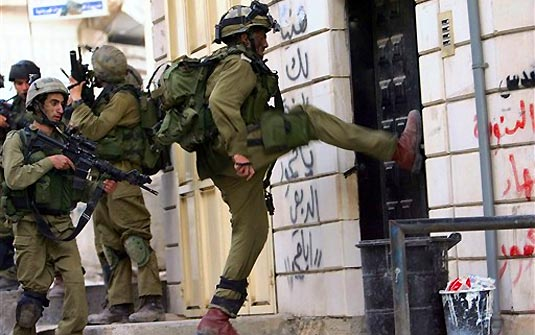
\includegraphics[width=\textwidth]{Escrita/penaporta}
  \end{center}
  \bigskip
  Vamos começar com um exemplo impactante...
\end{frame}

\begin{frame}{\small Esta frase é clara e de fácil compreensão?}
  \begin{exampleblock}{Exemplo}
    \footnotesize
    O tratamento com a droga, nas doses utilizadas aqui, que
    indicou aumento na sobrevivência e redução nos efeitos adversos,
    incluindo eventos SNC e não-SNC, teve eficácia
    comparável a outras drogas desta classe.
  \end{exampleblock}

  \begin{block}{Pergunta}
    \scriptsize
    Quanto tempo você precisa investir para compreender a informação que o autor quis transmitir?

    \bigskip

    Por que?
  \end{block}

  \vfill
  \scriptsize
  \hfill Fonte: Hindle, 2013.
\end{frame}

\begin{frame}{Estrutura $\times$ expectativa}
  Considere a seguinte lista de medições:
  \begin{exampleblock}{Exemplo}
    \scriptsize
    \begin{center}
    t(time)=15', T(temperature)=32$^o$C, t=0', T=25$^o$C; t=6',

    T=29$^o$C; t=3', T=27$^o$C; t=12', T=32$^o$C; t=9'; T=31$^o$C
  \end{center}
  \end{exampleblock}\pause

  \begin{block}{Pergunta}
    As temperaturas estão subindo, descendo, oscilando...?
  \end{block}
  \vfill
  \scriptsize
  \hfill Fonte: Gopen e Swan, 1990.
\end{frame}

\begin{frame}{Estrutura $\times$ expectativa}
  Considere a seguinte lista de medições:
  \begin{exampleblock}{Exemplo}
    \scriptsize
    \begin{center}
    t(time)=15', T(temperature)=32$^o$C, t=0', T=25$^o$C; t=6',

    T=29$^o$C; t=3', T=27$^o$C; t=12', T=32$^o$C; t=9'; T=31$^o$C
  \end{center}
  \end{exampleblock}

  \begin{itemize}
    \footnotesize
  \item Introduzir uma \alert{listagem} de informações de forma textual pode
    ser oneroso para o leitor
  \item Especialmente se as medições não seguem uma ordem razoável
  \end{itemize}
  \vfill
  \scriptsize
  \hfill Fonte: Gopen e Swan, 1990.
\end{frame}

\begin{frame}{Estrutura $\times$ expectativa}
  \begin{exampleblock}{Exemplo}
    \footnotesize
    \begin{center}
    \begin{tabular}{cc}
      time (min) & Temperature ($^o$C) \\
      0 & 25 \\
      3 & 27 \\
      6 & 29 \\
      9 & 31 \\
      12 & 32 \\
      15 & 32 \\
    \end{tabular}
  \end{center}
  \end{exampleblock}
  \begin{itemize}
    \footnotesize
  \item<1-> Mesmas informações
  \item Mais facilidade para a compreensão do leitor
  \item \alert{Contexto} (tempo) onde cada \alert{informação}
    (temperatura) pode ser interpretada
  \end{itemize}
  \vfill
  \scriptsize
  \hfill Fonte: Gopen e Swan, 1990.
\end{frame}

\begin{frame}{Violação da expectativa}
  \begin{exampleblock}{Exemplo}
    \footnotesize
    \begin{center}
    \begin{tabular}{cc}
      Temperature ($^o$C) & time (min) \\
      25 & 0 \\
      27 & 3 \\
      29 & 6\\
      31 & 9\\
      32 & 12\\
      32 & 15 \\
    \end{tabular}
  \end{center}
  \end{exampleblock}
  \begin{itemize}
    \footnotesize
  \item A \alert{ordem} das informações faz diferença.
  \item Como lemos da esquerda para a direita, preferimos:
    \begin{enumerate}
      \scriptsize
    \item contexto na esquerda
    \item novidades na direita
    \end{enumerate}
  \end{itemize}

  \vfill
  \scriptsize
  \hfill Fonte: Gopen e Swan, 1990.
\end{frame}

\begin{frame}{Exercício}
  O que esta figura quer dizer?
  \begin{center}
    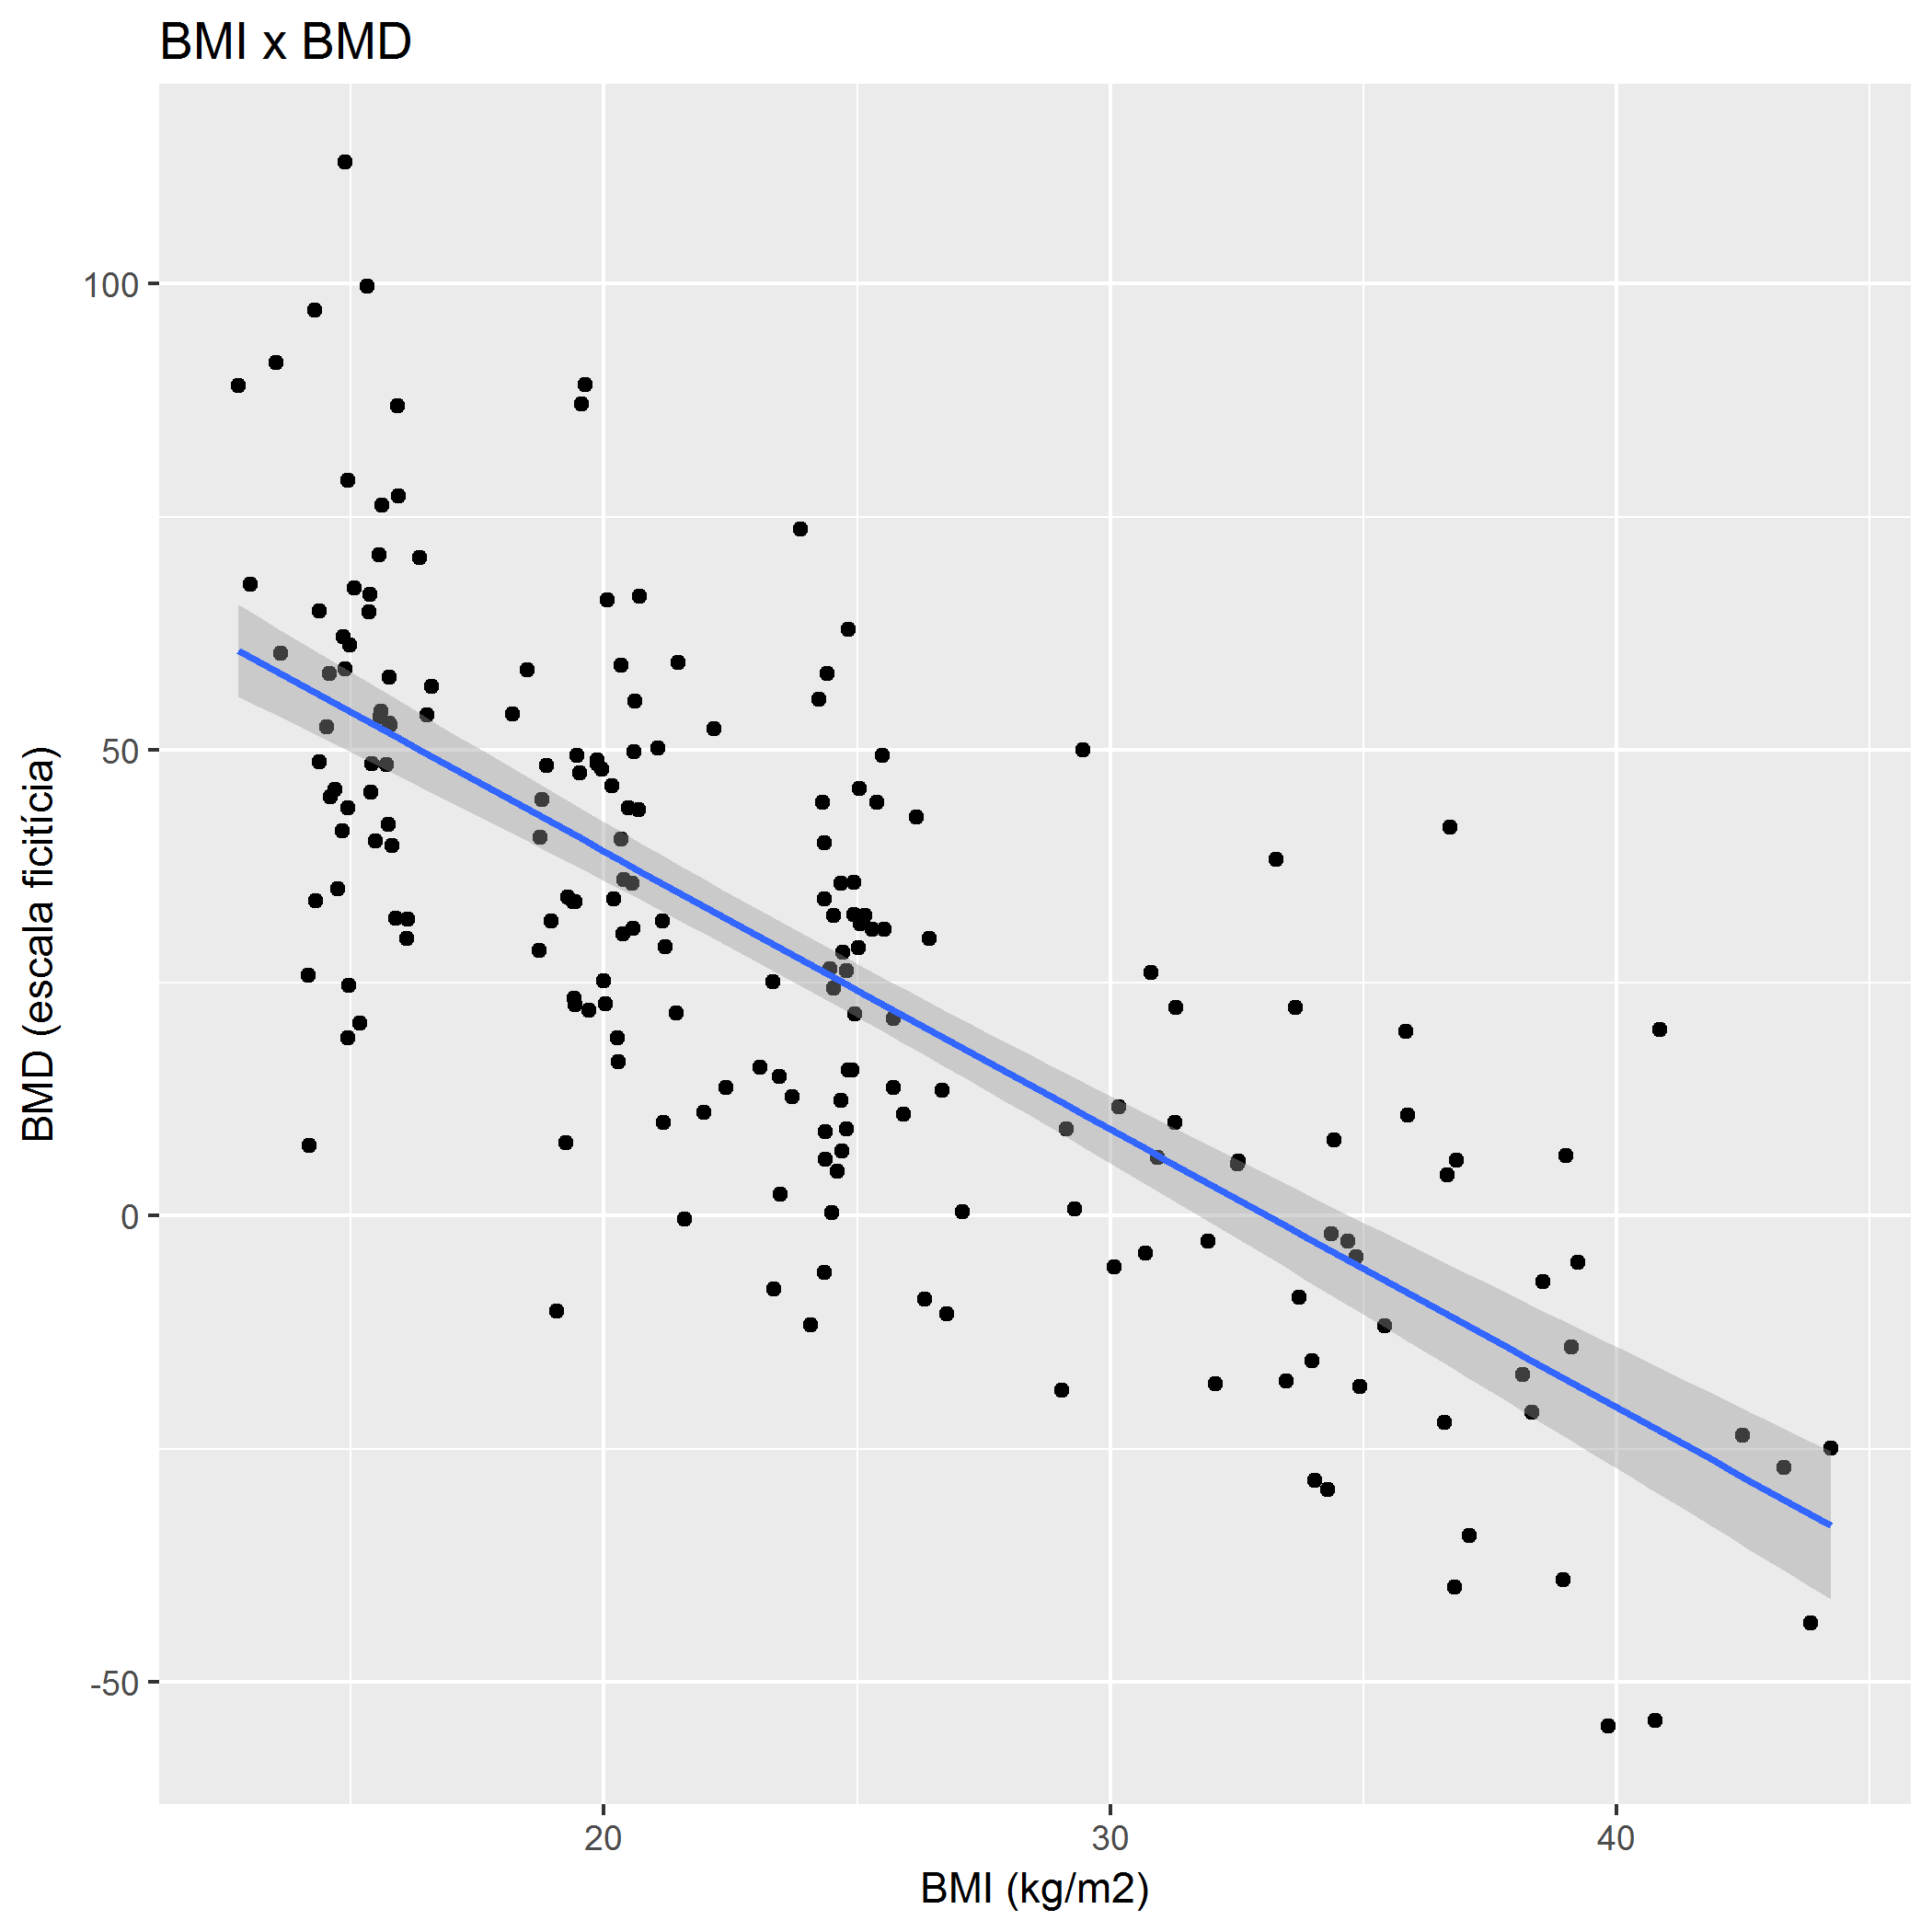
\includegraphics[height=.8\textheight]{Escrita/exercicio-figura}
  \end{center}
\end{frame}

\begin{frame}{Exercício 2}
  O que esta tabela quer dizer?
  \begin{center}
    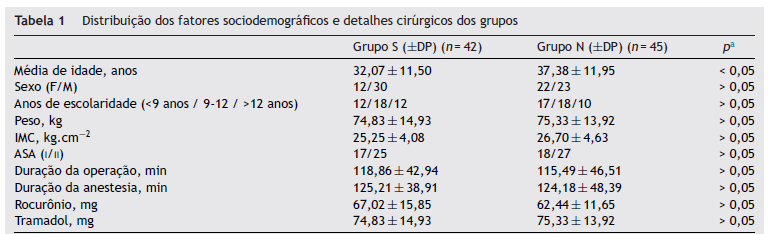
\includegraphics[width=1.18\textwidth]{Escrita/exercicio-tabela-1}
  \end{center}
\end{frame}

\begin{frame}{Exercício 2}
  Abreviações dos autores
  \begin{center}
    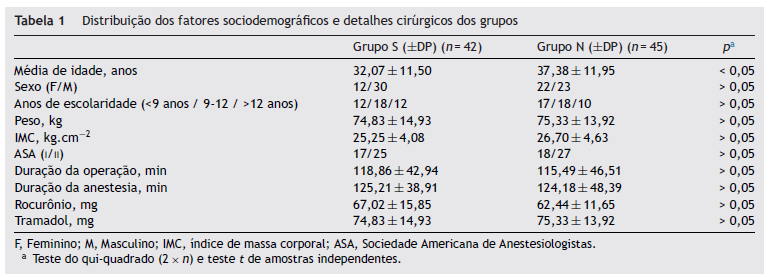
\includegraphics[width=1.18\textwidth]{Escrita/exercicio-tabela-2}
  \end{center}
\end{frame}

\begin{frame}{Contexto $\times$ novidade}
  \begin{itemize}
    \footnotesize
  \item Todo texto científico começa com a Introdução, e termina com
    as Conclusões
    \medskip
  \item Isto também deve se aplicar às unidades textuais menores:
    \visible<2->{
    \begin{enumerate}
      \scriptsize
    \item parágrafos
    \item frases
    \end{enumerate}
    }
    \medskip
  \item O início da frase deve familiarizar o leitor
    \medskip
  \item O final da frase deve intrigar o leitor
  \end{itemize}
\end{frame}

\begin{frame}{Expectativas do leitor}
  \begin{itemize}
    \footnotesize
  \item<1-> Unidades textuais grandes (tese, dissertação, artigo, livro):
    \alert<-2>{expectativa} de localizar informação nas respectivas
    seções
    \medskip
  \item<2-> Seções confusas (eg. muitos detalhes experimentais em
    Resultados): leitor igualmente confuso
    \medskip
  \item<3-> Unidades menores (seção, parágrafo, frase): divisões menos
    óbvias, \alert<3>{expectativas estruturais persistem}
    \medskip
  \item<4-> Violação das expectativas: o \alert{leitor precisa dedicar
      energia} para decifrar a estrutura usada
    \medskip
  \item<5-> Resultado: risco de interpretação errônea, ou não compreensão
  \end{itemize}

\vfill
Gopen e Swan, 1990.
\end{frame}

\begin{frame}{Resumo}
  \begin{block}{Gopen e Swan, 1990}
    A informação é interpretada mais facilmente e mais uniformemente
    se estiver posicionada onde a maior parte dos leitores espera
    encontrá-la.
  \end{block}
\end{frame}

\subsection{Distância entre verbo e sujeito}

\begin{frame}{Voltando ao primeiro exemplo}
  \begin{exampleblock}{Exemplo}
    \footnotesize
    O \alert<2>{tratamento com a droga}, nas doses utilizadas aqui, que
    indicou aumento na sobrevivência e redução nos efeitos adversos,
    incluindo eventos SNC e não-SNC, \alert<2>{teve} eficácia
    comparável a outras drogas desta classe.
  \end{exampleblock}

  \begin{block}{Pergunta}
    \scriptsize
    Esta frase é clara, de fácil compreensão?

    \bigskip
    Se não, por que não?
  \end{block}

  \vfill
  \scriptsize
  \hfill \href{https://web.archive.org/web/20150512001938/http://www.edanzediting.com/blog/reader_expectations_subject_verb_placement}
  {Hindle, 2013}
\end{frame}

\begin{frame}{Distância entre verbo e sujeito}
  \begin{exampleblock}{Exemplo}
    \scriptsize
    O \alert{tratamento com a droga}, nas doses utilizadas aqui, que
    indicou aumento na sobrevivência e redução nos efeitos adversos,
    incluindo eventos SNC e não-SNC, \alert{teve} eficácia
    comparável a outras drogas desta classe.
  \end{exampleblock}
  \uncover<2>{
  \begin{exampleblock}{Exemplo}
    \footnotesize
    Nas doses utilizadas aqui, o \alert{tratamento com a droga teve}
    eficácia comparável a outras drogas desta classe, que também
    indicou aumento na sobrevivência e redução nas taxas de efeitos
    adversos, incluindo eventos SNC e não-SNC.
  \end{exampleblock}
}

  \vfill
  \scriptsize
  \hfill \href{https://web.archive.org/web/20150512001938/http://www.edanzediting.com/blog/reader_expectations_subject_verb_placement}
  {Hindle, 2013}
\end{frame}

\subsection{A posição de ênfase}

\begin{frame}{A posição de ênfase}
  \begin{exampleblock}{Exemplo}
    \footnotesize
    Paul finalmente ganhou o prêmio depois de comprar 100 bilhetes de
    loteria \alert<2->{na loja}.
  \end{exampleblock}

  \visible<2>{
  \begin{block}{Pergunta}
    \footnotesize
    O que há de tão importante nesta loja??
  \end{block}
  }

  \vfill
  \scriptsize
  \hfill \href{http://serialmentor.com/blog/2013/9/26/writing-paragraphs-that-make-sensethe-topic-and-the-stress-position}
  {Wilke, 2013}
\end{frame}

\begin{frame}{A posição de ênfase}
  Reordenando a frase...
  \begin{exampleblock}{Exemplo}
    \footnotesize
      Paul teve que comprar 100 bilhetes de loteria até finalmente
      \alert<2->{ganhar o prêmio}.
  \end{exampleblock}
  \begin{itemize}
    \footnotesize
  \item A informação mais importante da frase é \alert{ganhar o
      prêmio}
  \item A loja nem foi mencionada (irrelevante)
  \end{itemize}


  \vfill
  \scriptsize
  \hfill \href{http://serialmentor.com/blog/2013/9/26/writing-paragraphs-that-make-sensethe-topic-and-the-stress-position}
  {Wilke, 2013}
\end{frame}

\subsection{A posição de tópico}

\begin{frame}{A posição de tópico}
  \begin{itemize}
    \footnotesize
  \item O início da frase indica o assunto a ser tratado
    \medskip
  \item Esta é chamada a \alert{posição de tópico} da frase
    \medskip
  \item Inverter a ordem das palavras altera o significado da frase
    (mudança de contexto)
  \end{itemize}
\end{frame}

\begin{frame}{A posição de tópico}
  \begin{exampleblock}{Exemplo}
    \footnotesize
    A \alert<2->{erosão do solo} é um problema sério nas regiões
    montanhosas do Nepal.
  \end{exampleblock}
  \begin{block}{Assunto}
    \footnotesize
    O assunto da frase acima é a \alert<2->{erosão do solo}.
  \end{block}

  \vfill
  \scriptsize
  \hfill \href{https://web.archive.org/web/20150512123007/http://www.edanzediting.com/blog/reader_expectations_topic_position}
  {Hindle, 2013}
\end{frame}

\begin{frame}{A posição de tópico}
  \begin{exampleblock}{Exemplo}
    \footnotesize
    As \alert<2->{regiões montanhosas do Nepal} encaram problemas sérios com o
    aumento da erosão do solo.
  \end{exampleblock}
  \begin{block}{Assunto}
    \footnotesize
    Esta estrutura indica que o assunto da frase é \alert<2->{uma
      região específica} do Nepal.
  \end{block}

  \vfill
  \scriptsize
  \hfill \href{https://web.archive.org/web/20150512123007/http://www.edanzediting.com/blog/reader_expectations_topic_position}
  {Hindle, 2013}
\end{frame}

\begin{frame}{Encadeamento de tópicos}
  \begin{itemize}
    \footnotesize
  \item Estrutura: cada idéia bem posicionada é mais fácil ser
    localizada
  \item Fluidez: conectar a ``nova idéia'' da frase anterior com o
    assunto da próxima frase
  \item ênfase (anterior) $\Rightarrow$ tópico (seguinte)
  \end{itemize}
\end{frame}

\begin{frame}{Encadeamento de tópicos -- frase}
  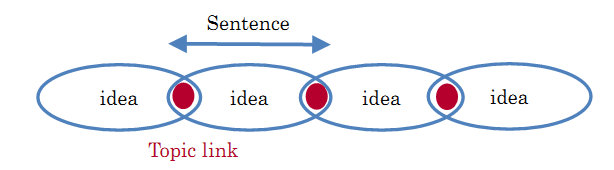
\includegraphics[width=\textwidth]{Escrita/encadeamento1}

  \vfill
  \scriptsize
  \hfill \href{https://web.archive.org/web/20150512123007/http://www.edanzediting.com/blog/reader_expectations_topic_position}
  {Hindle, 2013}
\end{frame}

\begin{frame}{Encadeamento de tópicos -- parágrafos}
    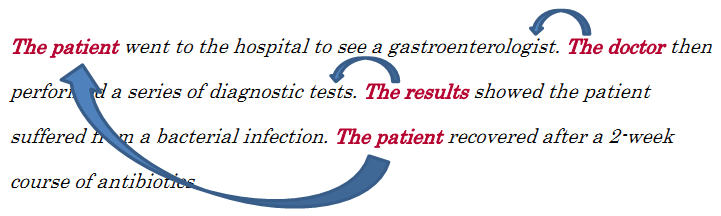
\includegraphics[width=\textwidth]{Escrita/encadeamento2}

  \vfill
  \scriptsize
  \hfill \href{https://web.archive.org/web/20150512123007/http://www.edanzediting.com/blog/reader_expectations_topic_position}
  {Hindle, 2013}
\end{frame}

\subsection{Voz ativa}

\begin{frame}{Voz passiva x ativa}
  \begin{exampleblock}{Exemplo}
    \footnotesize
    O tratamento com a droga, nas doses utilizadas aqui, que
    \alert<2>{indicou aumento} na sobrevivência e redução nos
      efeitos adversos, incluindo eventos SNC e não-SNC,
      \alert<2>{teve eficácia} comparável a outras drogas desta
      classe.

    % The drug treatment, at the doses used here, which provided improved survival and a decreased rate of adverse events, including CNS and non-CNS events, was found to have comparable efficacy to other drugs in this class.
  \end{exampleblock}
  \begin{block}{Perguntas}
    \begin{itemize}
      \footnotesize
    \item Qual é a ação executada? \visible<2>{(\alert{ações?})}
    \item Quem a executou?
    \end{itemize}
  \end{block}

  \vfill
  \scriptsize
  \hfill \href{https://web.archive.org/web/20150321052033/http://www.edanzediting.com/blog/reader_expectations_active_voice}
  {Hindle, 2013}
\end{frame}

\begin{frame}{Voz passiva x ativa}
  \begin{exampleblock}{Passiva}
    \scriptsize
    O tratamento com a droga, nas doses utilizadas aqui, que
    \alert{indicou aumento} na sobrevivência e redução nos efeitos adversos,
    incluindo eventos SNC e não-SNC, \alert{teve eficácia}
    comparável a outras drogas desta classe.

    % The drug treatment, at the doses used here, which provided improved survival and a decreased rate of adverse events, including CNS and non-CNS events, was found to have comparable efficacy to other drugs in this class.
  \end{exampleblock}
  \begin{exampleblock}{Ativa}
    \small
  \visible<2>{
    Nas doses utilizadas aqui, o tratamento com a droga \alert{teve eficácia} comparável a outras drogas desta classe.
    Este também \alert{indicou aumento} na sobrevivência e redução na taxa de efeitos adversos, incluindo eventos SNC e não-SNC.

    % At the doses used here, the drug treatment had comparable efficacy to other drugs in this class. It also provided improved survival and a decreased rate of adverse events, including CNS and non-CNS events.
}
  \end{exampleblock}

  \vfill
  \scriptsize
  \hfill \href{https://web.archive.org/web/20150321052033/http://www.edanzediting.com/blog/reader_expectations_active_voice}
  {Hindle, 2013}
\end{frame}

\subsection{Resumo}

\begin{frame}{Princípios estruturais}

  \begin{enumerate}
    \scriptsize
  \item Posicione o verbo \alert{após} o sujeito gramatical \alert{tão
      cedo quanto possível}
  \item Posicione a ``nova informação'' que você quer que o leitor
    enfatize na \alert{posição de ênfase}
  \item Posicione a pessoa ou coisa a que a frase se refere no início,
    na \alert{posição de tópico}
  \item Posicione qualquer ``informação antiga'' (que já foi
    discutida) na \alert{posição de tópico} para relacionar com o que
    passou e contextualizar com o que virá
  \item Articule a ação de cada frase em seu verbo (\alert{voz ativa})
  \item Em geral, indique algum contexto para seu leitor antes de
    exigir que ele considere qualquer informação nova
  \item Em geral, tente assegurar que as ênfases relativas do conteúdo
    coincidem com as expectativas relativas levantadas pela estrutura
  \end{enumerate}
\end{frame}

\begin{frame}{Tutorial (editora Springer)}
  \begin{center}
    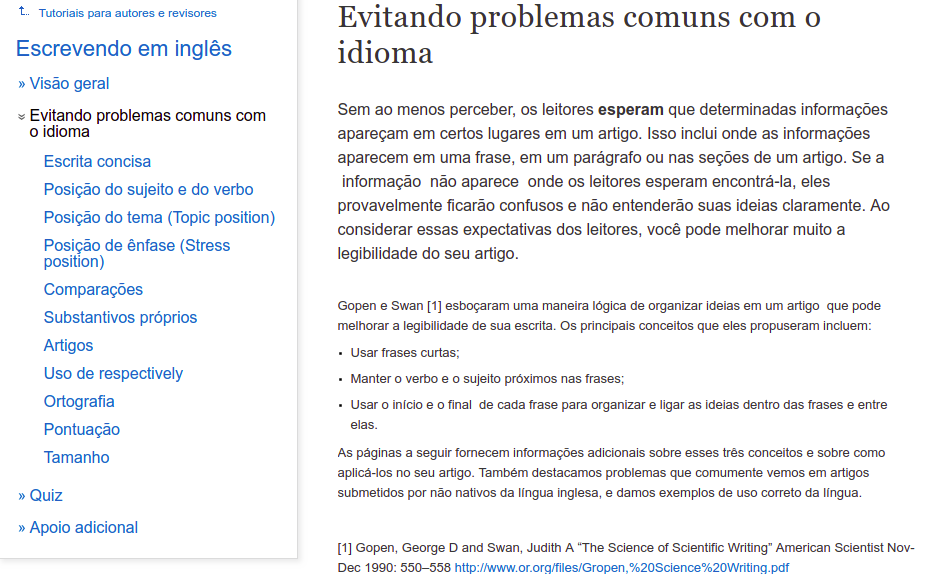
\includegraphics[width=.9\textwidth]{Escrita/springer-tutorial}
  \end{center}
  \vfill \scriptsize \hfill
  \href{https://www.springer.com/br/authors-editors/authorandreviewertutorials/writinginenglish/avoiding-common-language-issues/12012044}
  {Springer -- Tutoriais para autores e revisores}
\end{frame}

\section{Aprofundamento}

\subsection{Aprofundamento}

\begin{frame}{Aprofundamento}
  \begin{block}{Leitura obrigatória}
    \footnotesize
    \href{https://www.georgegopen.com/uploads/1/0/9/0/109073507/gopen___swan_sci_of_sci_writing_am_sci_1990_.pdf}
    {GOPEN, George D.; SWAN, Judith A. The science of scientific writing. {\bf American Scientist}, v. 78, n. 6, p. 550-558, 1990.}
  \end{block}
  \begin{block}{Leitura recomendada}
    \begin{itemize}
      \tiny
    \item
      \href{http://serialmentor.com/blog/2013/9/26/writing-paragraphs-that-make-sensethe-topic-and-the-stress-position}
      {Wilke, Claus. Writing paragraphs that make sense, 2013} {\tiny (acessado em 20/10/2015)}.
    \item
      \href{https://web.archive.org/web/20150512085221/http://www.edanzediting.com/blog/tag/reader_expectations}
      {Hindle, Amanda. Reader expectations (blog series), 2013} {\tiny (acessado em 20/10/2015)}.
      \begin{itemize}
        \tiny
      \item
        \href{https://web.archive.org/web/20150512001938/http://www.edanzediting.com/blog/reader_expectations_subject_verb_placement}
        {Reader expectations -- Subject \& verb placement}
      \item
        \href{https://web.archive.org/web/20150321052033/http://www.edanzediting.com/blog/reader_expectations_active_voice}
        {Reader expectations -- Active voice}
      \item
        \href{https://web.archive.org/web/20150511225632/http://www.edanzediting.com/blog/reader_expectations_stress_position}
        {Reader expectations -- Stress position}
      \item
        \href{https://web.archive.org/web/20150512123007/http://www.edanzediting.com/blog/reader_expectations_topic_position}
        {Reader expectations -- Topic position}
      \item
        \href{https://web.archive.org/web/20150512003347/http://www.edanzediting.com/blog/reader_expectations_sentence_length}
        {Reader expectations -- Sentence length}
      \end{itemize}
    \item
      \url{http://www.phrasebank.manchester.ac.uk/} {\tiny (acessado em 27/03/2019)}.
    \item
      \href{https://www.springer.com/br/authors-editors/authorandreviewertutorials/writinginenglish/avoiding-common-language-issues/12012044}
      {Springer -- Tutoriais para autores e revisores} {\tiny(acessado em 31-03-2019)}
    \end{itemize}
  \end{block}
\end{frame}

\end{document}
